\section{Accuracy of current methods for predicting roll damping}
\label{se:accuracy_SI_method}
Some studies for instance \parencite{soder_assessment_2019} show that the Ikeda's method is not capable to accurately predict the roll damping for some modern ship cases. The SI-method being the simplified version of Ikeda's method most likely inherits its problems but also introduces some extrapolation errors as reported by \parencite{rudakovic_application_2017}. In the following, 227 existing roll decay model tests conducted at SSPA Maritime Dynamics Laboratory are used to validate the SI-method. The comparison will help to identify the drawbacks and improvement potentials of the SI-method. It aims at further developing this method to increase its accuracy based on the large test database through some statistical regression analysis.

Prior to the validation the behaviour of the SI-method was studied by varying the input parameters between minimum and maximum values in database around a point "reference ship" with values in the middle of the input boundaries (Eq. \ref{eq:SI_limits}) (see figure \ref{fig:SI_sensitivity}). It can be seen that the wave damping $B_W$ increases a lot with the absolute value of $OG/T$. It can also be seen the the wave damping has an enormous increase when the beam to draught ratio exceeds the input boundary, which seems to be the case for at least one third of the roll decay tests. It can also be noted that most of the ships in the database have midsection coefficients $A_0$ and bilge keel heights that exceed the limit. 

\begin{figure}[H]
    \centering
    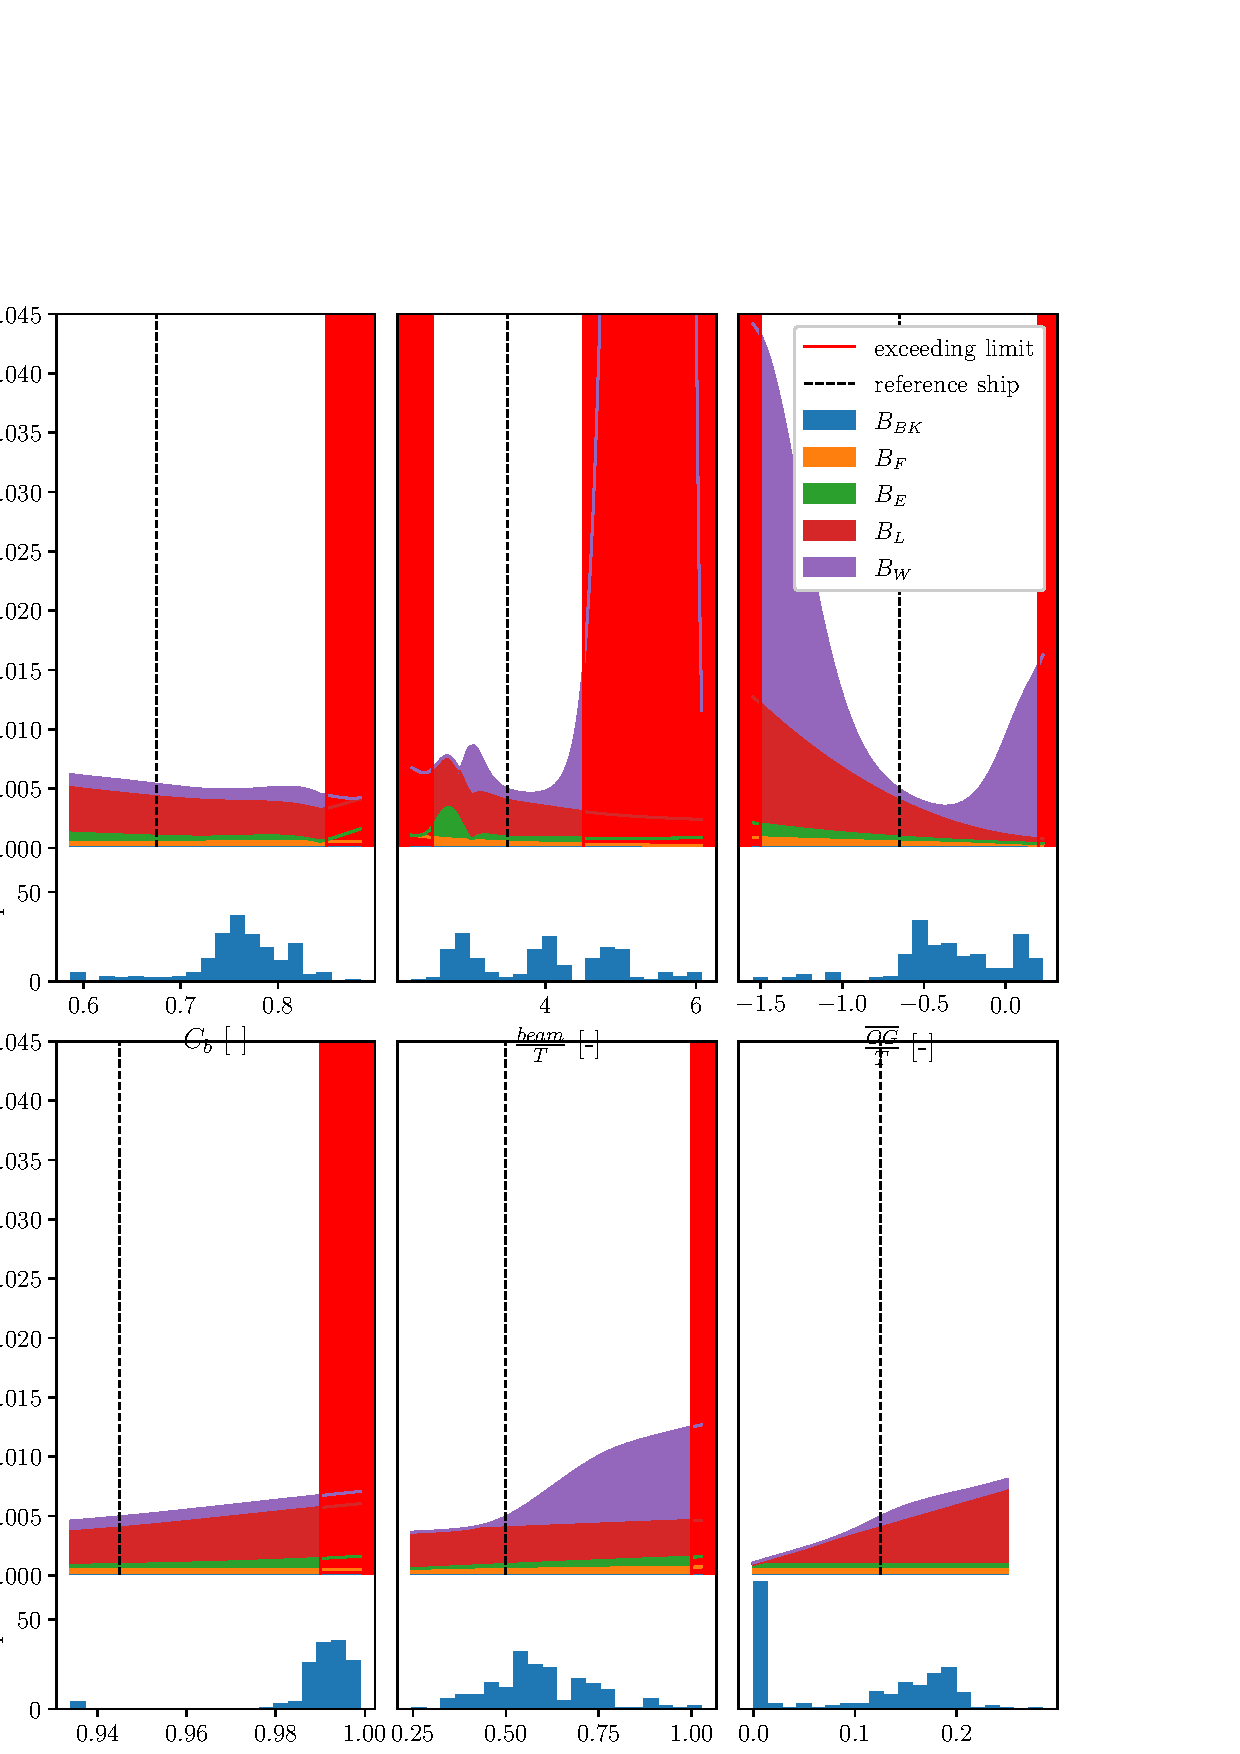
\includegraphics[width=6in, height = 8in ]{figures/SI-sensitivity.pdf}
        \vspace{-0.5cm}
    \caption{SI-method input parameter variation and data base ships}
    \label{fig:SI_sensitivity}
\end{figure}

\subsection{Overall accuracy of Ikeda\'s method}
\label{se:overall_comparison}
In the following, we will present an overall comparison between Ikeda\'s method and the damping estimated from experimental test database in order to identify possible potential to improve Ikeda\'s method.


Figure \ref{fig:B_e_hat_ikeda} shows a comparison of the nondimensional equivalent linear damping from model tests and the simplified method.  

\begin{figure}[H]
    \centering
    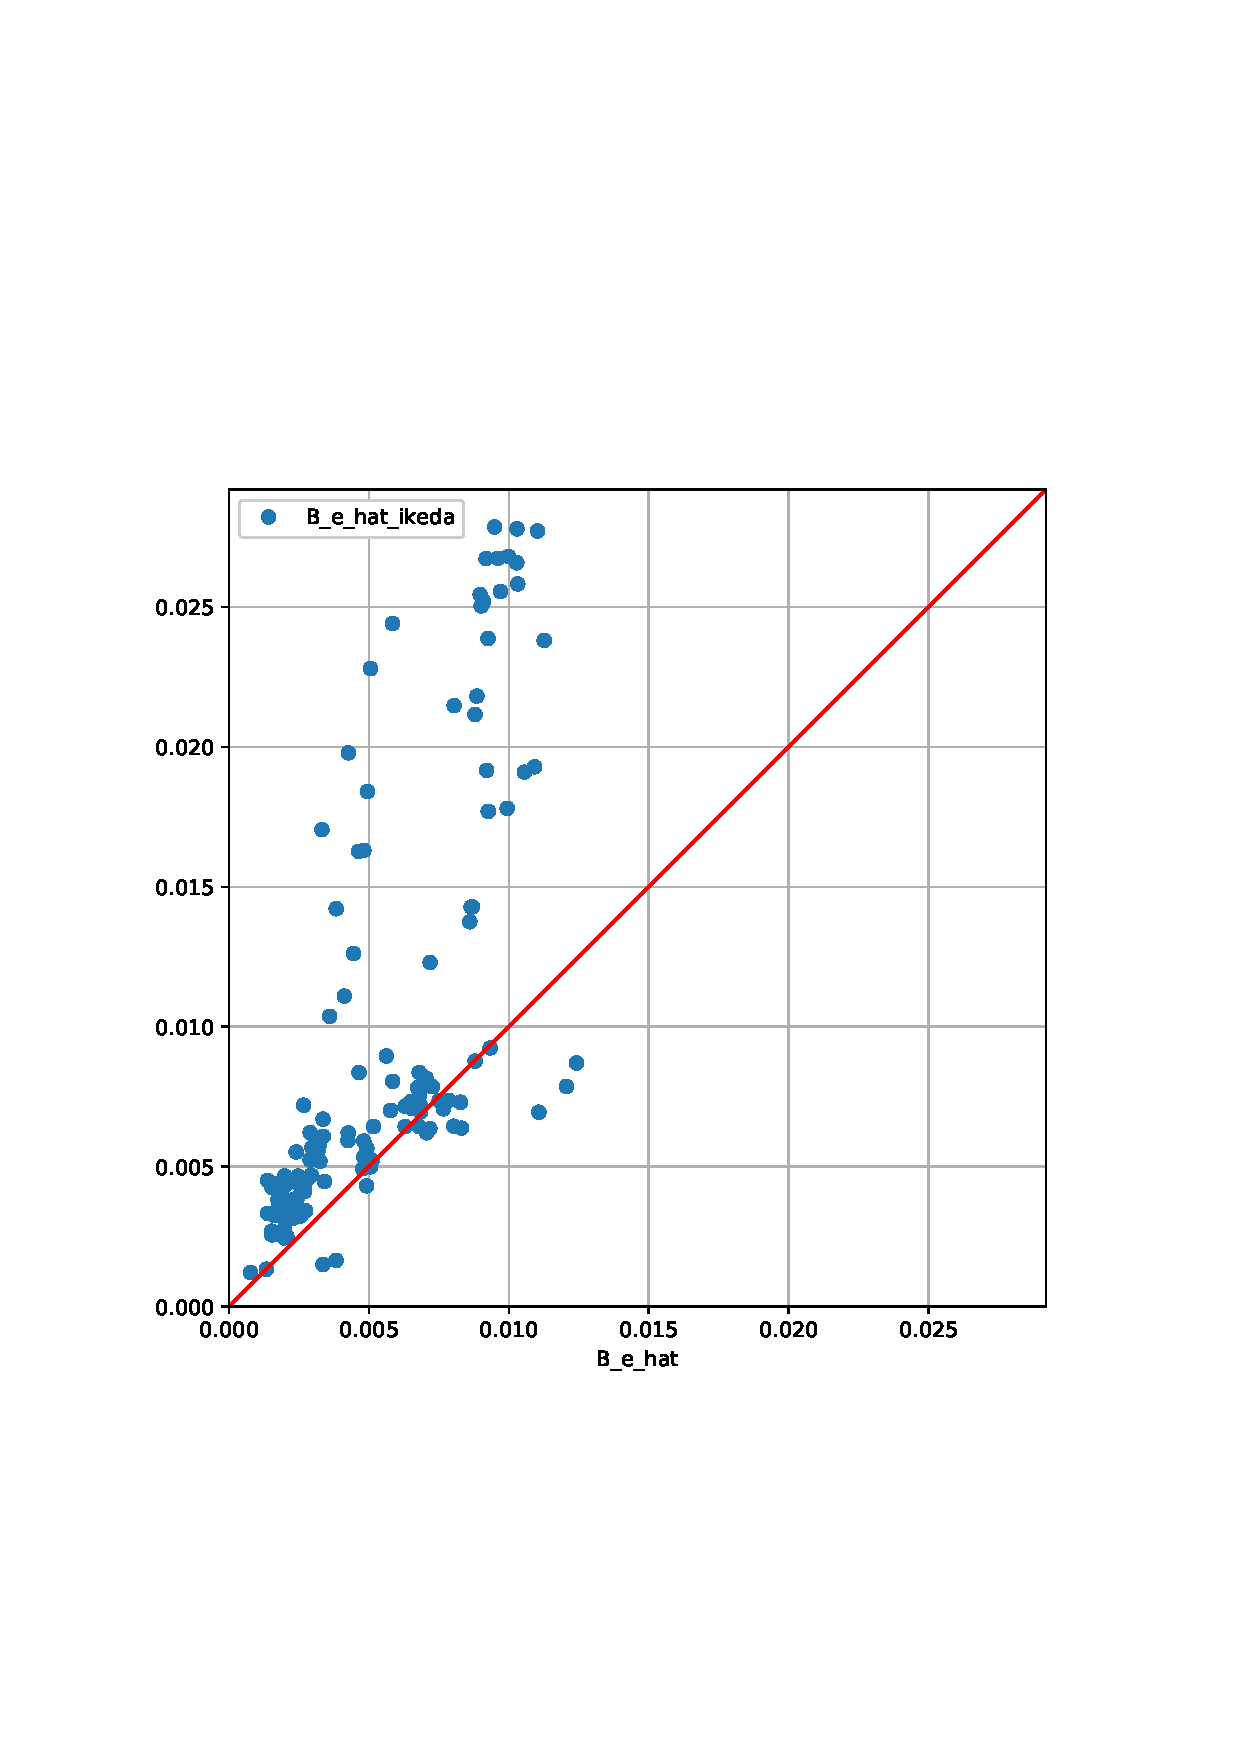
\includegraphics[width=\columnwidth]{figures/B_e_hat_ikeda.pdf}
    \caption{Nondimensional linearized damping from model tests and simplified Ikeda}
    \label{fig:B_e_hat_ikeda}
\end{figure}

When plotting the error between the model test and simplified Ikeda method in figure \ref{fig:B_e_hat_error} this shows that the error is much larger for $T/L_{pp}<0.034$

\begin{figure}[H]
    \centering
    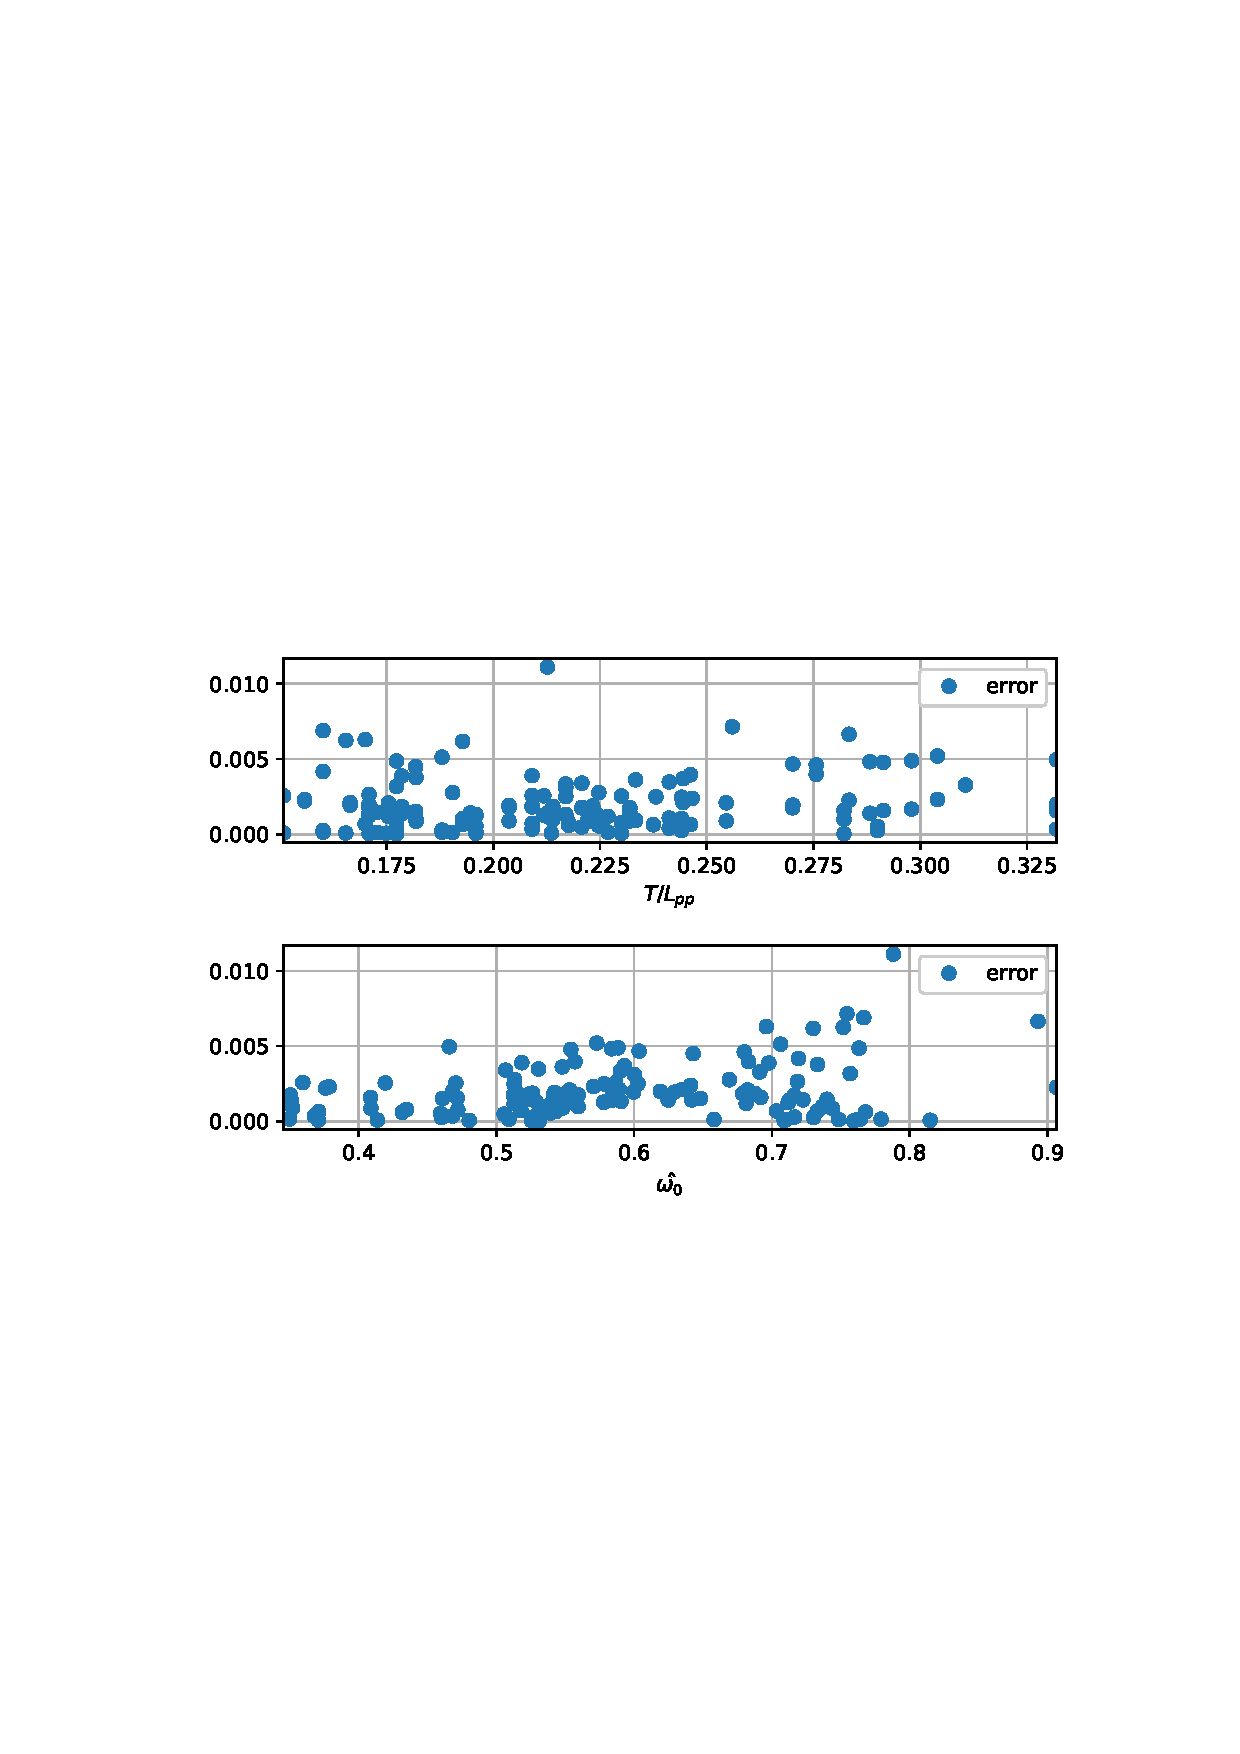
\includegraphics[width=\columnwidth]{figures/B_e_hat_error.pdf}
    \caption{Simplified Ikeda error versus draught}
    \label{fig:B_e_hat_error}
\end{figure}

Figure \ref{fig:B_e_hat_good} shows the comparison for only model tests with $T/L_{pp}>0.034$.
This confirms the small draft to beam ratio limit of this method as mentioned in \cite{kawahara_simple_2011}. The corresponding $R^2$ score is 0.38.

\begin{figure}[H]
    \centering
    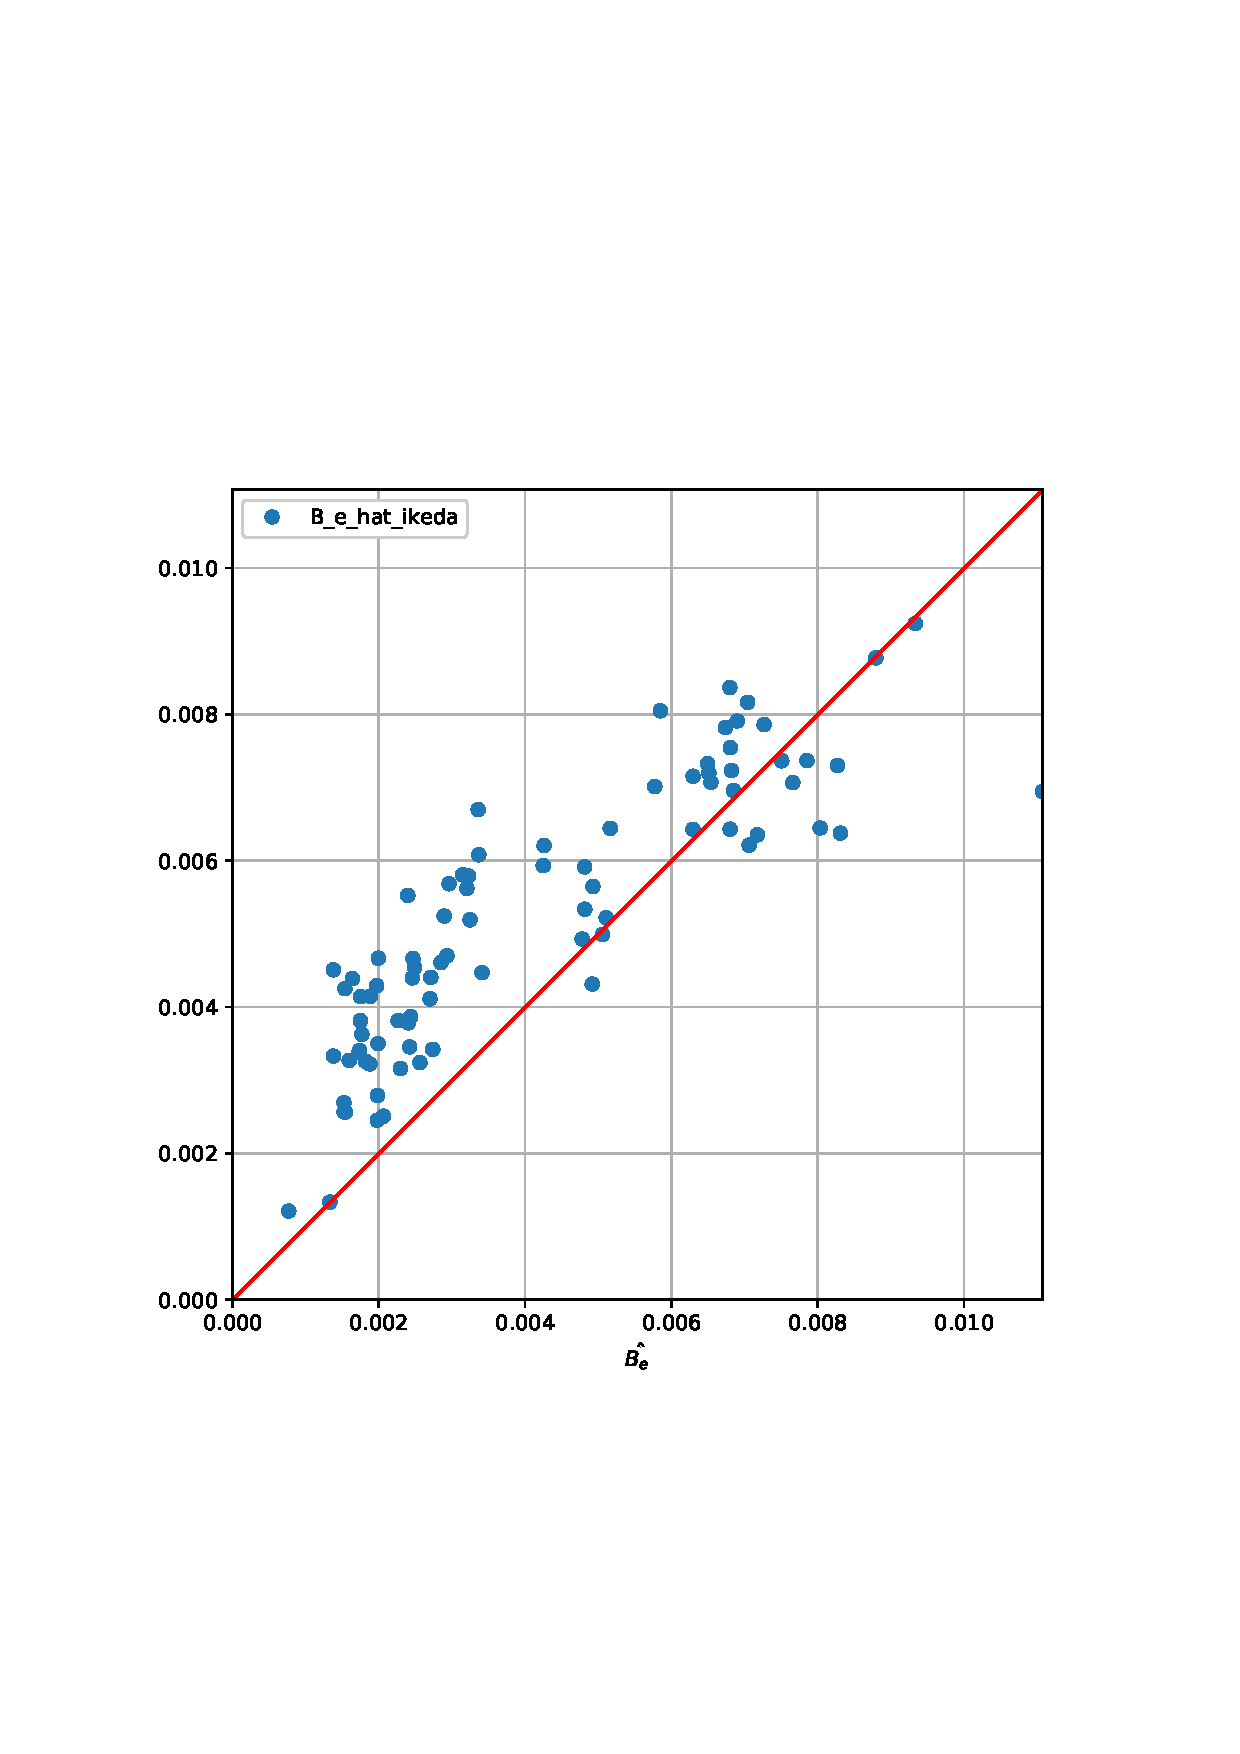
\includegraphics[width=\columnwidth]{figures/B_e_hat_good.pdf}
    \caption{Nondimensional linearized damping from model tests and simplified Ikeda $T/L_{pp}>0.034$}
    \label{fig:B_e_hat_good}
\end{figure}
